\documentclass[a4paper,12pt]{article}
\usepackage{times}
\usepackage[francais]{babel}
\usepackage[utf8x]{inputenc}
\usepackage[T1]{fontenc}
\usepackage{amsmath}
\usepackage{amssymb}
\usepackage{graphicx}
\usepackage{pdfpages}
\usepackage{pdflscape}
\usepackage{listings}
\usepackage{longtable}
\usepackage{float}

\lstset{literate=
{é}{{\'e}}1
{è}{{\`e}}1
{ê}{{\^e}}1
{à}{{\`a}}1
{â}{{\^a}}1
}
\lstset{language=C++,
                basicstyle=\footnotesize,
                keywordstyle=\footnotesize\color{blue},
                otherkeywords={override,nullptr}
}
\definecolor{orange}{rgb}{0.8,0.4,0.0}
\definecolor{darkblue}{rgb}{0.0,0.0,0.6}
\definecolor{cyan}{rgb}{0.0,0.6,0.6}
\lstdefinelanguage{JSON}
{
  basicstyle=\normalsize,
  columns=fullflexible,
  showstringspaces=false,
  commentstyle=\color{gray}\upshape,
  morestring=[b]",
  morestring=[s]{>}{<},
  morecomment=[s]{<?}{?>},
  stringstyle=\color{orange},
  identifierstyle=\color{darkblue},
  keywordstyle=\color{blue},
  morekeywords={string,number,array,object}% list your attributes here
}

\sloppy

\setlength{\topmargin}{0cm}
\setlength{\headsep}{0.in}
\setlength{\headheight}{0.in}
\setlength{\evensidemargin}{0cm}
\setlength{\oddsidemargin}{-1cm}
\textwidth 18cm
\textheight 25cm

\begin{document}

\thispagestyle{empty}

\begin{titlepage}

\vspace*{2cm}

\begin{center}\textbf{\Huge Projet Logiciel Transversal}\end{center}{\Large \par}

\begin{center}\textbf{\large Mohamed KHLIFI et Ihsen OUERGHI}\end{center}{\large \par}

\vspace{2cm}

%\begin{figure}[h]
%\begin{center}
%\includegraphics[width=\textwidth]{exemple.png}
%\caption{\label{pacmangame}Exemple du jeu}
%\end{center}
%\end{figure}

\clearpage

{\small
\tableofcontents
}

\end{titlepage}

\clearpage
\section{Présentation Générale}

\subsection{Archétype}

\vspace{1\baselineskip}


Le jeu que  nous souhaitons réaliser consiste en une opposition entre 2 joueurs dans la conquête d’une map. Notre jeu s’appuie ainsi sur les archétypes des jeux Total War et Civilization. 

Au départ les deux joueurs se voient confier un nombre égal de ressources et une ville, le reste de la map restant caché pour l'instant. Dès lors, les deux joueurs vont devoir explorer la map, par l'intermédiaire d'un type de joueur (nommé explorateur), se développer et conquérir de nouveaux territoires. Des combats peuvent survenir pour la conquête d'une ville, ceux-ci seront simulés et donneront lieu à un vainqueur qui remportera la ville.

Le jeu se finit lorsque l'un des joueurs conquièrent toute la map.
\\

Notre jeu mêlera donc gestion/expansion de territoire, gestion de matières premières et gestion de ressources humaines.
Le jeu comporte une map principale découpée en plusieurs villes. Au départ celles-ci sont inhabitées et chaque joueur peut les coloniser. Concernant les personnages, nous commencerons avec deux types différents : les explorateurs et les soldats. Les explorateurs servent à coloniser des villes pour pouvoir les contrôler. Les soldats servent aux combats et déterminent en bonne partie l'issue de ceux-ci.


\subsection{Règles du jeu}

\vspace{1\baselineskip}


Une ville possède deux états : inhabitée ou colonisée. 

Une ville ne peut être colonisée que par des explorateurs.

Chaque ville possède deux notes : défense et fertilité. La note de défense est conditionnée par le nombre de soldats et par les fortifications construites. 

Chaque joueur possède deux ressources : la nourriture et l'or.
Si une ville est déjà colonisée par l'adversaire, il faut l'attaquer pour la conquérir.

Les combats sont simulés et prennent en compte l'armée qui attaque d'un côté et la note de la ville et l'armée qui défend de l'autre.
\\

Les bâtiments disponibles sont : \begin{itemize}

\item Fermes et mines pour les ressources

\item Caserne et fortifications pour produire les soldats et la note de défense

\item Hôtel de ville pour produire les explorateurs

\end{itemize}


\subsection{Ressources}

\vspace{1\baselineskip}


Pour les ressources nous avons trouvé pour démarrer un tileset minimaliste mais largement suffisant pour réaliser ce que nous avons en tête simplement. Il a été ajouté au dossier res du projet.
\\

\begin{figure}[H]
\begin{center}
  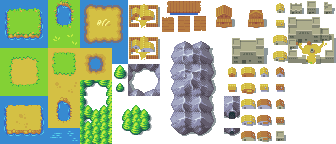
\includegraphics[width=0.7\textwidth]{images/tileset.png}
  \caption{Tileset pour la map}
 \end{center}

\end{figure}

Nous avons aussi besoin de sprites représentant les armées et les exportateurs, pour cela nous avons trouvé en ligne un éditeur de personnages que nous avons adapté pour l'IA et le joueur.

\begin{figure}[H]
\begin{center}
  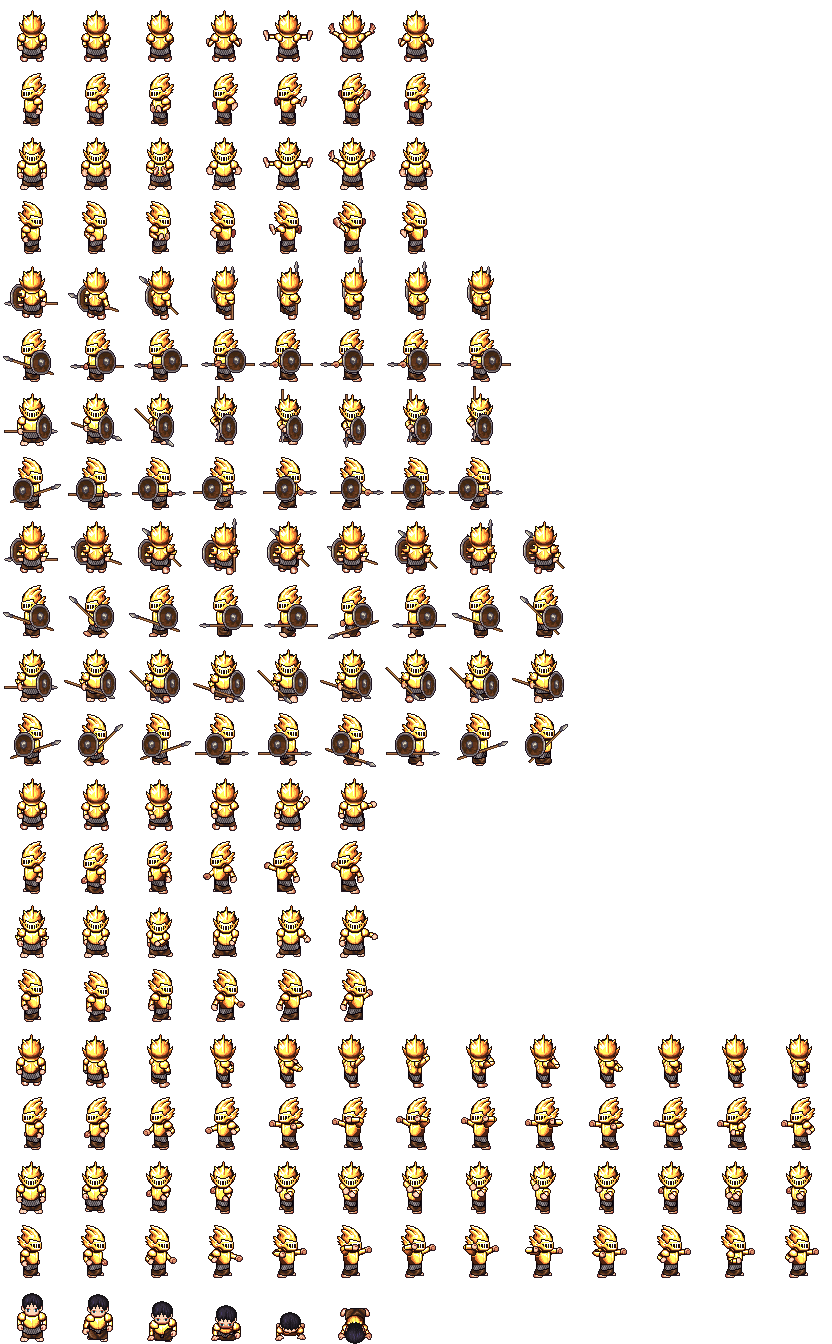
\includegraphics[width=0.7\textwidth]{images/Army_Gold.png}
  \caption{Armée du joueur}
 \end{center}
\end{figure}

\begin{figure}[H]
\begin{center}
  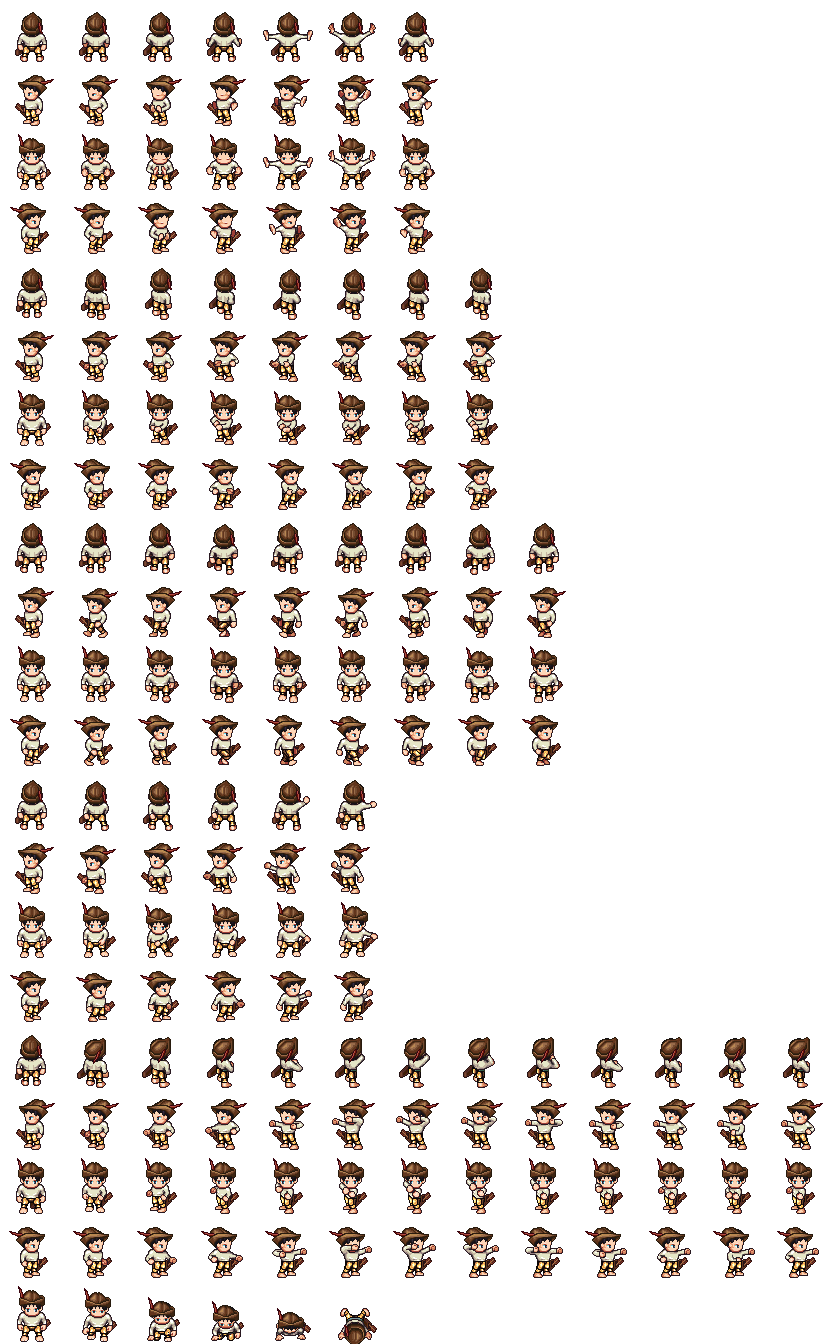
\includegraphics[width=0.7\textwidth]{images/Settlers_Gold.png}
  \caption{Explorateurs du joueur}
 \end{center}
\end{figure}

\begin{figure}[H]
\begin{center}
  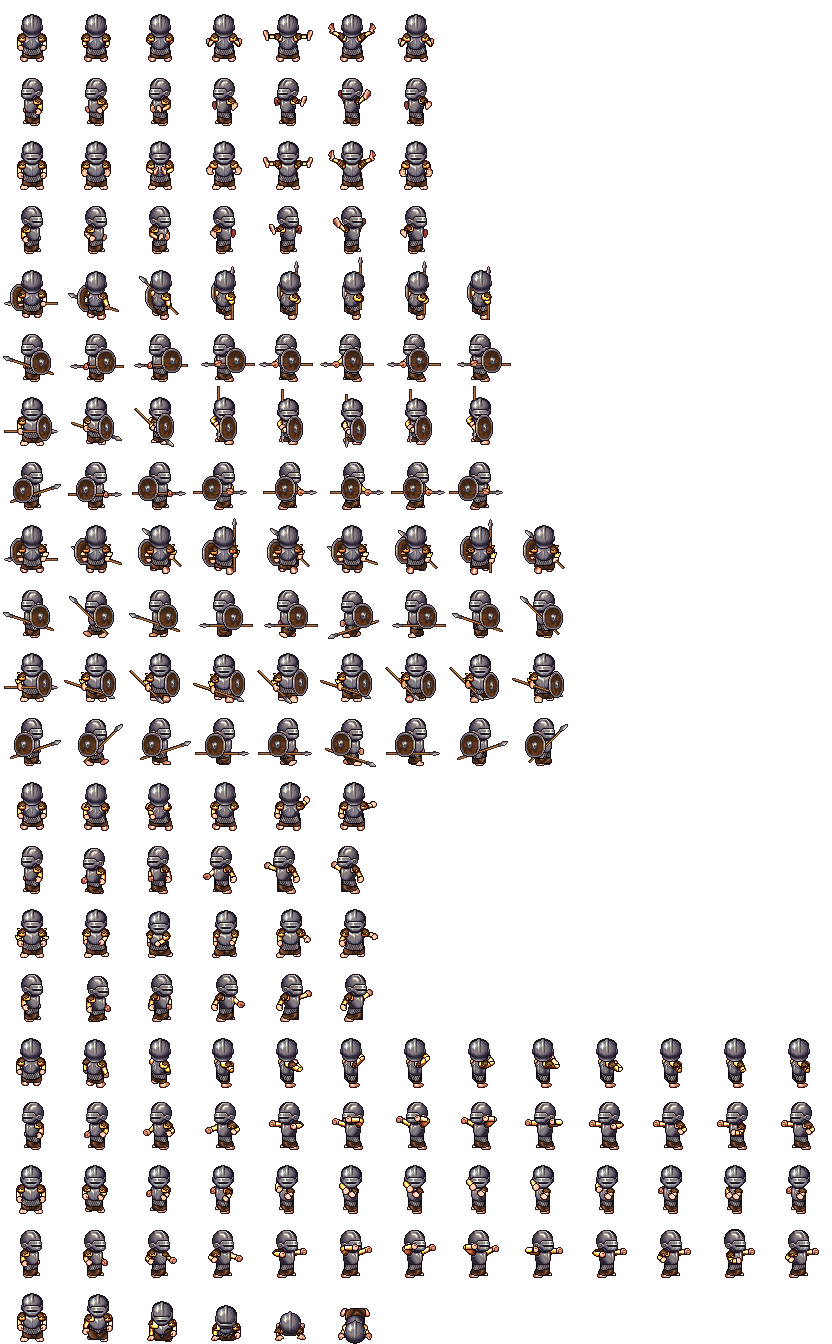
\includegraphics[width=0.7\textwidth]{images/Army_Silver.png}
  \caption{Armée de l'IA}
 \end{center}
\end{figure}

\begin{figure}[H]
\begin{center}
  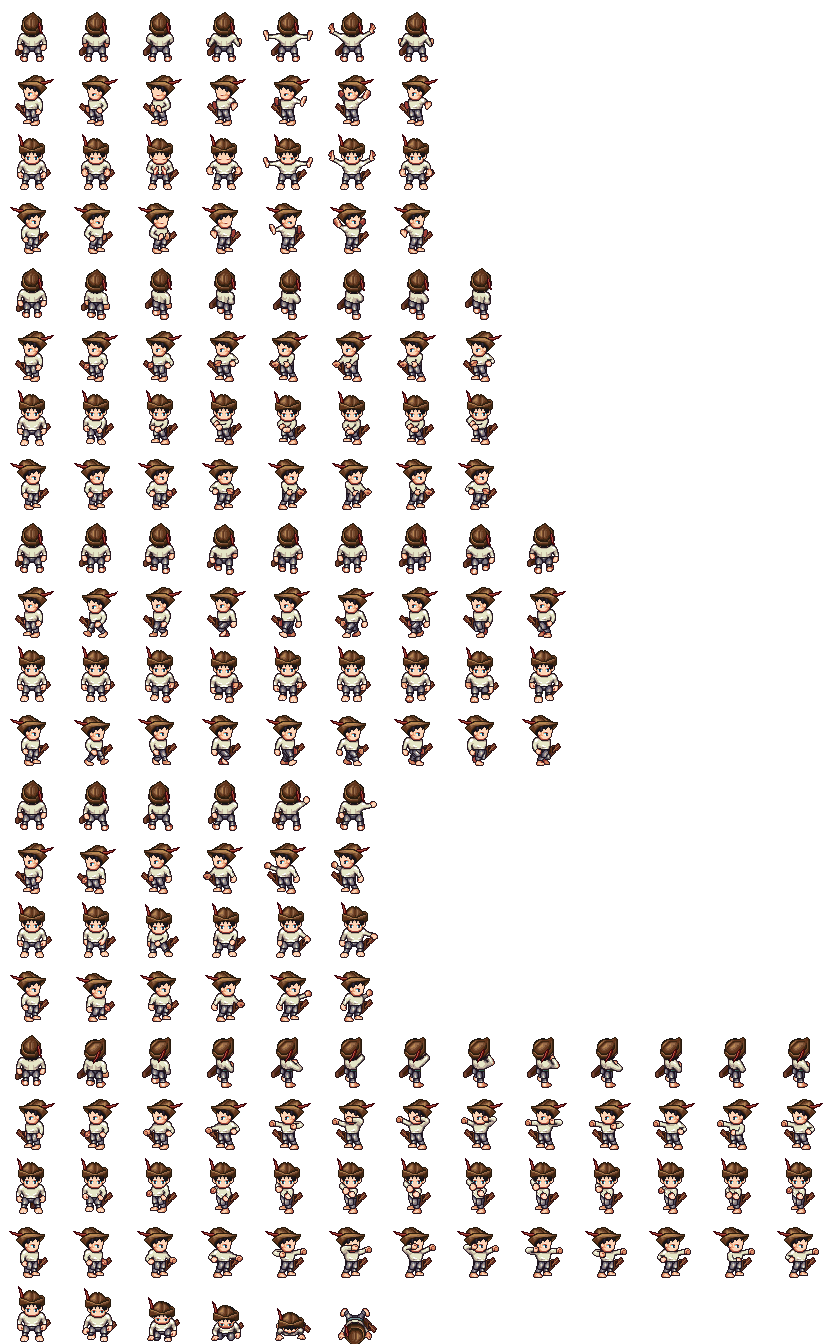
\includegraphics[width=0.7\textwidth]{images/Settlers_Silver.png}
  \caption{Explorateurs de l'IA}
 \end{center}
\end{figure}

Bien sur certaines animations du spritesheet ne seront pas utilisées.

\clearpage

\section{Description et conception des états}

\subsection{Description des états}

Notre jeu sera constitué d'une map principale sur laquelle se déroule tout le jeu. Au départ, nous prévoyons que le joueur ne connaisse qu'une partie de celle-ci, l'idée étant de s'aventurer sur la map pour pouvoir la découvrir. Ceci implique ainsi de ne connaître ni les positions des villes, ni la position initiale du joueur adversaire au départ.
Il y aura des éléments fixes et mobiles, ceux ci auront une position, et appartiendront à un des joueurs.

\subsubsection{États à éléments fixes}


\textbf{Cases "City" : } chaque ville possède un nombre de cases déterminé sur lesquelles elle va se construire.
\\
Nous avons aussi une classe Construction (pour bâtiment). Une City possède un tableau de constructions. Trois classes héritent de Construction : Mine (pour l'extraction de l'or), Farm (pour la production de nourriture) et Barrack (pour la création de soldats). Cette City peut être en état de construction ou non, elle peut être libre ou non. 
\\
%/\begin{tabular}{llll}
 %/      Nous avons aussi une classe Construction (pour bâtiment) qui hérite de la classe City, et qui hérite elle-même de trois nouvelles classes :&
%/       Mine : pour l'extraction d'or\\
  %/    Farm : pour la fabrication de nourriture\\
    %/  Barrack (caserne) : pour la création de soldats
     
%/\end{tabular}/%
%/\begin{tabular}{lllll}
 %/   & Nous avons aussi une classe Construction (pour bâtiment) qui hérite de la classe City, et qui hérite elle-même de trois nouvelles classes : &  \\
  %/ 2.1 & 2.2 & 2.3 \\
   %/2.1 & 2.2 & 2.3 \\
   %/2.1 & 2.2 & 2.3
%/\end{tabular}

\textbf{Cases "Landscape" :} cases en dehors des villes dans lesquelles peuvent se déplacer les explorateurs et les soldats. Dans la classe correspondante, chaque Landscape peut être accessible ou non pour les éléments mobiles.
\\
\subsubsection{États à éléments mobiles}

\textbf{Élément "Army" :} Unité de combat pour la défense d'une ville et pour la conquête armée de territoire. Elle peut attaquer une ville déjà conquise ou les éléments adversaires hors des villes : \begin{itemize}

\item si elle rencontre un groupe de soldat : simulation du combat

\item si elle rencontre des explorateurs, elle les tue.
\\
\end{itemize}
Elles peuvent être en garnison dans une ville ou bien en déplacement sur la carte.

\textbf{Élément "Settlers" :} Unité d'exploration et d'expansion. Permet de découvrir la map, et des colonies dans les villes inhabitées. Cette unité précieuse dans l'expansion est complètement impuissante contre les soldats et meure si elle se fait attaquer.

\subsubsection{États général}

L'état général est défini par les époques, ainsi que le joueur qui est en train de jouer.


\subsection{Conception Logicielle}

Le diagrame UML est donné ds la prochaine figure, les principales classes sont Element et ses heritières.
Ensuite la classe Player, et enfin la classe monde, contenant une grille d'éléments.

\begin{figure}[H]
\begin{center}
  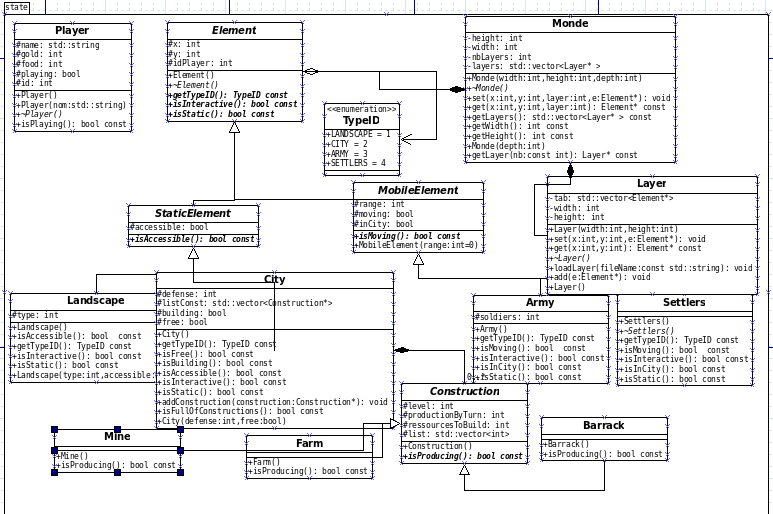
\includegraphics[width=1\textwidth]{images/stateUML.png}
  \caption{Diagramme UML des états}
 \end{center}

\end{figure}
\clearpage
\section{Rendu: Stratégie et Conception}

\subsection{Stratégie de rendu d'un état}

Pour réaliser notre rendu nous sommes partis d'un tileset que nous avons édité grâce au logiciel Tiled. Celui-ci permet de dessiner des maps à partir d'un tileset importé. A partir de celui disponible en figure 1, nous l'avons découpé en pixels de 16x16 grâce à Tiled et avons dessiné plusieurs maps pour la suite du projet.
\\Dans un premier nous sommes partis sur trois maps : \begin{itemize}
\item Une map "Obstacles"pour les test que nous réaliserons plus tard, assez basique pour l'instant
\item Une map "Montagne" qui s'appuie principalement sur les éléments de roche du tileset
\item Une map "Mer" qui s'appuie principalement sur les éléments marins du tileset.
\end{itemize}

Pour réaliser toutes ces maps, nous choisissons de découper chaque map en plusieurs couches ou "layers" qui regroupent des informations ou éléments différents. Ainsi, notre premier layer correspond à l'arrière plan et se compose exclusivement d'herbe verte, et est donc commun à toutes les maps. Le deuxième layer nous sert à définir la map : suivant la map à éditer on aura tel ou tel paysage, la superposition des deux premiers layers donnera donc "naissance" à une map vierge. Le troisième layer nous servira pour la gestion des éléments mobiles, à savoir les explorateurs et les armées. Enfin nous prévoyons un quatrième layer pour l'interface utilisateur qui regroupera les informations du jeu, les interactions avec les objets du jeu, ... Ce dernier layer sera précisé et conçu par la suite. 
Une fois ces cartes dessinés on exporte au format CSV chaque layer de la carte. Ainsi à chaque démarrage du jeu, on aura la possibilité d'initialiser les états pour les éléments fixes à partir des fichier CSV correspondant aux layer, et d'un autre fichier CSV contenant une matrice permettant de transformer directement un tile en état. 
Ensuite durant le jeu, nous réaliserons le rendu directement à partir des états.

\subsection{Conception logicielle}

\textbf{RenderLayer.}
 Cette classe charnière va nous permettre de concevoir le rendu visuel de notre jeu et s'appuie notamment sur les classes MapLayer et CharacterLayer qui héritent de celle-ci MapLayer contient les deux premières couches d'éléments fixes composant le niveau, et CharactersLayers contient les éléments mobiles de la troisieme couche. Ces deux dernières classes initialisent les vecteurs 2D qui préparent le rendu à afficher. En effet ce sont ces classes qui sont reliés aux états, on peut ainsi créer le rendu à partir des états directement. 
 \\
 
\textbf{Drawer.}
Cette classe va charger les textures, elle va aussi initialiser et configurer les vecteurs par l'intermédiaire des méthodes initVertex, setVertexLocation et setVertexTexture. Cette classe fait aussi le lien avec SFML pour afficher les textures à l'écran. On affiche le rendu grâce aux tableaux de vertex, ainsi cette classe comprend le tableau de vertex qui stocke les quads, ainsi que la texture.
\\

\textbf{Tileset.} 
Cette classe et ses filles se chargent des tiles, on a créé une classes génériques appelé Tile, permettant de créer une représentation des éléments du tileset, on stocke notamment la taille des éléments du tileset la position dans le tileset. MapSet permet de stocker un vecteur de tile, mais aussi la taille du tileset et le nom du fichier, et CharactersSet fait de même pour les personnages. Mais surtout c'est dans ces classes que se trouve la fonction getTile, qui permet de transformer un Élément en entité graphique que l'on peut afficher. 



\begin{figure}[H]
\begin{center}
  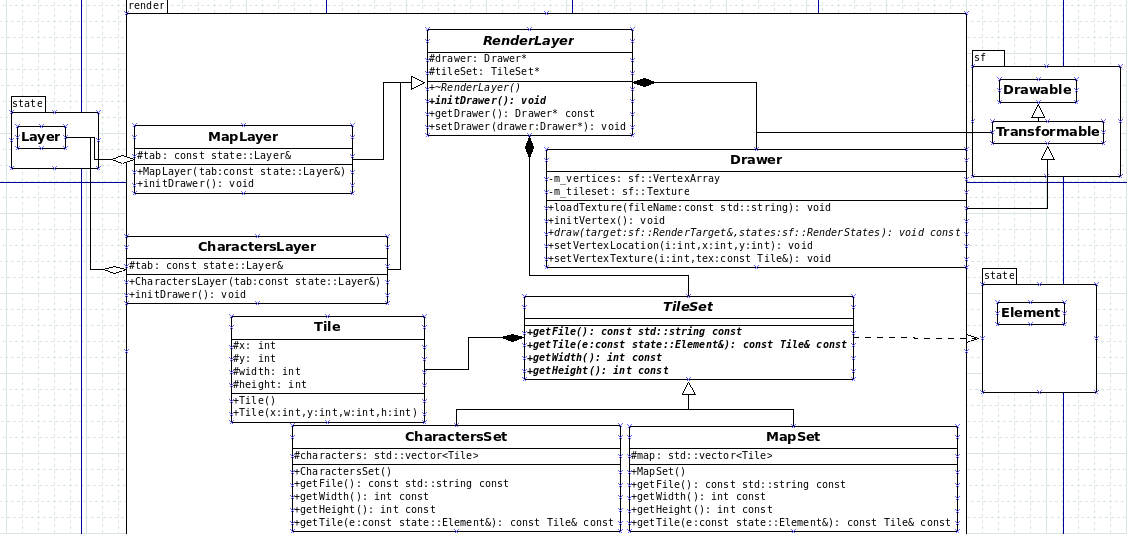
\includegraphics[width=1\textwidth]{images/UML_Render.png}
  \caption{Diagramme UML du rendu}
 \end{center}
 \end{figure}
 
%\begin{landscape}
%\begin{figure}[p]
%\includegraphics[width=0.9\paperheight]{render.pdf}
%\caption{\label{uml:render}Diagramme des classes de rendu.} 
%\end{figure}
%\end{landscape}



\end{document}